\section{Marco Te\'orico del prototipo}

\subsection{Online Grooming}
El online Grooming es un fen\'omeno que podr\'iamos traducir como engatusamiento y que se utiliza para describir las pr\'acticas online de ciertos adultos para ganarse la confianza de un (o una) menor fingiendo empat\'ia, cariño, etc. con fines de satisfacción sexual (como m\'inimo, y casi siempre, obtener im\'agenes del menor desnudo o realizando actos sexuales).

Por tanto est\'a muy relacionado con la pederastia y la pornograf\'ia infantil en Internet. De hecho el grooming es en muchas ocasiones la antesala de un abuso sexual \cite{grooming}.

\subsection{Caracterización del online grooming}
De acuerdo a las conversaciones analizadas por los Doctores Aditi Gupta, Ponnurangam Kumaraguru, Ashish Surekason del Instituto Tecnol\'ogico de Informaci\'on en la India reportadas en el art\'iculo  ``Characterizing pedophile conversations on the Internet using Online Grooming Web.'' \cite{articulo}, identificaron una serie de etapas y estados que las  las conversaciones pueden atravesar. Los autores marcan 6 etapas principales las cuales se describen en la tabla \ref{table:caracterizacion}.


\begin{table}[!h]

\begin{tabular}[t]{|p{15mm} |p{22mm} |p{22mm} |p{22mm} |p{20mm} |p{20mm} |p{20mm} |}
\hline
\hline
Etapas & Formaci\'on de la amistad & Formaci\'on de una relaci\'on & Evaluaci\'on de riesgos & Exclusividad & Sexual & Conclusi\'on \\
\hline
Descriptor1 & Intercambio de cuentas de correo electr\'onico, fotograf\'ias, webcam, informaci\'on & Intercambio de cuentas de correo electr\'onico, fotograf\'ias, webcam, informaci\'on & Evaluar a los padres del ni\~no, si est\'an alrededor o qui\'en puede ver su computadora & Sentir amor y expresar exclusividad & Dar descripci\'on del cuerpo y la figura & Quedar un d\'ia, una cita, hora, lugar para conocerse en persona \\
\hline
Descriptor2 &Hablar de novios/novias & Dar suaves cumplidos & Pedir al ni\~no eliminar su historial de conversaciones, asegurarse quenadie tenga la contrase\~na & Describir actividad sexual y experiencias al ni\~no &Ser novios &Discutir puntos en com\'un para una reuni\'on \\
\hline
Descriptor3 &Obtener informaci\'on del perfil y otras cuentas del ni\~no & hablar de los hobbies del a\~no, actividades e intereses & Ver si el ni\~no est\'a c\'omodo con ver a alguien mayor& Cumplidos fuertes & Intercambiar fotograf\'ias sexuales & Asegurarse de que el ni\~no ir\'a s\'olo \\
\hline
Descriptor4 & Preguntar la edad, genero, localidad, nombre, informaci\'on personal, detalles familiares & Escuela, grado, tareas, n\'umero de celular & Asegurarse de que el ni\~no no es un polic\'ia & Construir confianza entre el ni\~no y el ped\'ofilo & Dar orientaci\'on sexual, cumplidos & Decidir qu\'e hacer cuando se conozcan\\
\hline
\end{tabular} \\ \\ \\
\caption{Tabla de caracterizaci\'on del comportamiento de conversaciones peligrosas}
\label{table:caracterizacion}
\end{table}

%Con base a la tabla de caracterizacion del comportamiento de las conversaciones se propuso un conjunto de frases de acuerdo a la etapa que 
%A partir de la observaci\'on de las conversaciones y de acuerdo con la descripci\'on de la matriz se listan las siguientes frases, las cuales marcan un punto de inter\'es en la identificaci\'on de los niveles 1, 2, 3, 4 y 6:



\subsection{Lista de frases de nivel 1}
La siguiente lista de frases pertenecen al nivel 1 de caracterizaci\'on, cuyo objetivo es establecer confianza y obtener datos de la v\'ictima. Estas frases fueron seleccionadas en relaci\'on a que en la observaci\'on al momento de traducir las conversaciones est\'as aparec\'an con mayor frecuencia.

\begin{itemize}
\item ?`C\'omo te llamas?
\item ?`C\'ual es tu nombre?
\item ?`Cu\'antos a\~nos tienes?
\item ?`D\'onde vives?
\item ?`Qu\'e m\'usica te gusta?
\end{itemize}


\subsection{Lista de frases de nivel 2}
La siguiente lista de frases son frases que pertenecen al nivel 2 de caracterizaci\'on, cuyo objetivo es establecer amistad con la v\'ictima. Al igual que las frases del nivel anterior estas fueron seleccionadas debido a su frecuente apari\'on medida en la observaci\'on al momento de traducir las conversaciones.


\begin{itemize}
\item ?`Tienes Fotos?
\item ?`Tienes webcam?
\item ?`En qu\'e escuela vas?
\item ?`Cu\'al es tu celular?
\item ?`Cu\'al es tu tel\'efono?
\item ?`Cu\'al es tu n\'umero telef\'onico?
\end{itemize}




\subsection{Lista de frases de nivel 3}
La siguiente lista de frases son frases que pertenecen al nivel 3 de caracterizaci\'on, cuyo objetivo es conocer la situaci\'on y relacion de la v\'ictima con sus padres o familiares. 


\begin{itemize}
\item ?`D\'onde est\'a tu mam\'a?
\item ?`D\'onde est\'a tu pap\'a?
\item ?`Tus pap\'as trabajan?
\end{itemize}


\subsection{Lista de frases de nivel 4}
La siguiente lista de frases son frases que pertenecen al nivel 4 de caracterizaci\'on, cuyo objetivo es establecer vinculos de novizago o alg\'un tipo de relaci\'on. 


\begin{itemize}
\item ?`Quieres ser mi novia?
\item ?`Quieres ser mi novio?
\item Eres bonita o bonito.
\item Eres guapo.
\item Me gustas. 
\item Eres hermosa.
\end{itemize}

\subsection{Lista de frases de nivel 6}
La siguiente lista de frases son frases que pertenecen al nivel 6. Este nivel tiene como objetivo establecer contacto con la v\'ictima, haciendo citas o alg\'un tipo de reuni\'on. Al igual que los niveles anteriores las frases seleccionadas aqu\'i fueron seleccionadas de acuerdo a una selecci\'on basada en la observaci\'on de las conversaciones traducidas.


\begin{itemize}
\item Quiero verte
\item ?`D\'onde nos vemos?
\item Te veo en este lugar.
\item Hay que reunirnos.
\end{itemize}

Hacemos menci\'on del nivel 5 cuya caracter\'istica es la descripci\'on sexual de las conversaciones. Este nivel ser\'a evaluado por separado en el prototipo n\'umero 2 ya que el contexto sexual da un peso mayor en la desici\'on de la API.
\textbf{•}

\section{Descripci\'on}
Prototipo que identifica y cuenta frases pertenecientes a los niveles de  formaci\'on de la amistad, formaci\'on de una relaci\'on, evaluaci\'on de riesgos, exclusividad y conclusi\'on de la caracterizac\'on del online grooming.

\section{Objetivo}
Desarrollar un prototipo que procese conversaciones de texto para buscar y contar las frases de los niveles de formaci\'on de la amistad, formaci\'on de una relaci\'on, evaluaci\'on de riesgos, exclusividad y conclusi\'on descritas en la tabla de caracterizac\'on del online grooming.


\section{An\'alisis}
\subsection{Caracter\'istcas}

\begin{description}
\item[FEAT1:] El sistema realiza la b\'usqueda de frases del nivel de formaci\'on de amistad.
\item[FEAT2:] El sistema raliza el conteo de frases del nivel formaci\'on de amistad.
\item[FEAT3:] El sistema realiza la b\'usqueda de frases del nivel formaci\'on de una relaci\'on.
\item[FEAT4:] El sistema raliza el conteo de frases del nivel formaci\'on de una relaci\'on.
\item[FEAT5:] El sistema realiza la b\'usqueda de frases del nivel de evaluaci\'on de riesgos.
\item[FEAT6:] El sistema raliza el conteo de frases del nivel evaluaci\'on de riesgos.
\item[FEAT7:] El sistema realiza la b\'usqueda de frases del nivel de exclusividad.
\item[FEAT8:] El sistema raliza el conteo de frases del nivel de exclusividad.
\item[FEAT9:] El sistema realiza la b\'usqueda de frases del nivel de conclusi\'on.
\item[FEAT10:] El sistema raliza el conteo de frases del nivel conclusi\'on.
\end{description}

\subsection{Restricciones}
\begin{itemize}
\item Conversaciones alamacenadas en archivos de texto planos.
\item Conversaciones almacenadas en archivos con formato XML.
\item Implementaci\'on del prototipo en python.

\end{itemize}

\section{Dise\~no}

La figura \ref{fig:arquitectura_prototipo2} muestra la arquitectura del prototipo. Tal como se muestra en el diagrama, la entrada de informaci\'on del prototipo son los archivos que contienen a las conversaciones. La salida del prototipo ser\'an los valores del n\umero de frases correspondientes a cada nivel de caracterizaci\'on del Online grooming. Estos valores ser\'a almacenada en una base da datos para su posterioir procesamiento.



	\begin{figure}[!h]
	\begin{center}
	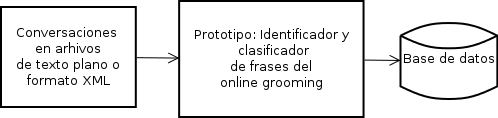
\includegraphics[scale=.5]{images/arquitectura_prototipo1}
	\caption{Arquitectura del prototipo 1}
	\label{fig:arquitectura_prototipo2}
	\end{center}
	\end{figure}


\subsection{Diagrama de Clases}


La figura \ref{fig:diagramaDeClase} muestra el diagrama de clase correspondiente a estre prototipo. En este diagrama los atributos: FrasesNivel1, FrasesNivel2, FrasesNivel3, FrasesNivel6, FrasesNivel6 hacen referencia al n\'umero de incidencias que el objeto conversacion tiene. Los m\'etodos: getValueNivel1(), getValueNivel2(), getValueNivel3(), getValueNivel4(), getValueNivel6() devuelven el atributo al cual este asociado.
	\begin{figure}[h]
	\begin{center}
	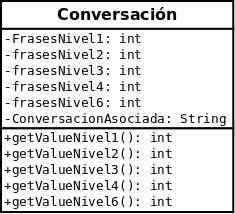
\includegraphics[scale=.4]{images/claseprotipo2}
	\caption{Diagrama de Clase del prototipo 1}
	\label{fig:diagramaDeClase}
	\end{center}
	\end{figure}
\section{Pruebas}


Se realizo una prueba de 50 conversaciones peligrosas y 50 peligrosas donde se obtivieron los resultadas mostrados en la tabla \ref{table:resultadosNiveles}



\begin{center}
\begin{longtable}{|l|l|l|l|l|l|}

\hline
Conversaci\'on & Nivel 1 & Nivel 2 & Nivel 3 & Nivel 4 & Nivel 6 \\
\hline
\endfirsthead

\hline
Conversaci\'on & Nivel 1 & Nivel 2 & Nivel 3 & Nivel 4 & Nivel 6 \\
\hline
\endhead

\multicolumn{5}{c}{Sigue en la página siguiente.}
\endfoot

\endlastfoot

conversaciones\_txt/8.txt & 2 & 3 & 1 & 0 & 0 \\
\hline
conversaciones\_txt/29.txt & 0 & 0 & 2 & 3 & 2 \\
\hline
conversaciones\_txt/31.txt & 0 & 0 & 1 & 3 & 0 \\
\hline
conversaciones\_txt/6.txt & 1 & 2 & 3 & 2 & 0 \\
\hline
conversaciones\_txt/25.txt & 4 & 4 & 5 & 0 & 0 \\
\hline
conversaciones\_txt/cp4.txt & 0 & 1 & 2 & 0 & 1 \\
\hline
conversaciones\_txt/cp2.txt & 2 & 7 & 10 & 3 & 1 \\
\hline
conversaciones\_txt/15.txt & 0 & 0 & 0 & 0 & 1 \\
\hline
conversaciones\_txt/38.txt & 1 & 0 & 8 & 1 & 1 \\
\hline
conversaciones\_txt/40.txt & 0 & 0 & 1 & 0 & 1 \\
\hline
conversaciones\_txt/34.txt & 0 & 3 & 0 & 1 & 0 \\
\hline
conversaciones\_txt/7.txt & 0 & 2 & 1 & 2 & 0 \\
\hline
conversaciones\_txt/20.txt & 1 & 0 & 0 & 0 & 2 \\
\hline
conversaciones\_txt/cp6.txt & 0 & 1 & 5 & 3 & 3 \\
\hline
conversaciones\_txt/9.txt & 0 & 1 & 3 & 0 & 0 \\
\hline
conversaciones\_txt/13.txt & 0 & 0 & 2 & 0 & 1 \\
\hline
conversaciones\_txt/4.txt & 1 & 1 & 1 & 1 & 1 \\
\hline
conversaciones\_txt/cp3.txt & 2 & 3 & 14 & 0 & 2 \\
\hline
conversaciones\_txt/23.txt & 1 & 1 & 1 & 0 & 0 \\
\hline
conversaciones\_txt/cp1.txt & 0 & 3 & 7 & 1 & 0 \\
\hline
conversaciones\_txt/36.txt & 0 & 2 & 8 & 1 & 0 \\
\hline
conversaciones\_txt/3.txt & 0 & 1 & 0 & 0 & 0 \\
\hline
conversaciones\_txt/cp7.txt & 0 & 7 & 5 & 1 & 2 \\
\hline
conversaciones\_txt/22.txt & 0 & 0 & 1 & 0 & 0 \\
\hline
conversaciones\_txt/26.txt & 0 & 0 & 0 & 1 & 0 \\
\hline
conversaciones\_txt/32.txt & 0 & 0 & 0 & 0 & 0 \\
\hline
conversaciones\_txt/21.txt & 0 & 0 & 0 & 2 & 0 \\
\hline
conversaciones\_txt/11.txt & 0 & 1 & 2 & 0 & 0 \\
\hline
conversaciones\_txt/30.txt & 1 & 2 & 4 & 0 & 0 \\
\hline
conversaciones\_txt/39.txt & 0 & 1 & 1 & 0 & 0 \\
\hline
conversaciones\_txt/1tx.txt & 2 & 4 & 0 & 1 & 3 \\
\hline
conversaciones\_txt/18.txt & 1 & 1 & 6 & 0 & 1 \\
\hline
conversaciones\_txt/28.txt & 0 & 0 & 3 & 0 & 0 \\
\hline
conversaciones\_txt/14.txt & 0 & 1 & 0 & 0 & 1 \\
\hline
conversaciones\_txt/12.txt & 0 & 0 & 0 & 0 & 1 \\
\hline
conversaciones\_txt/5.txt & 0 & 0 & 0 & 0 & 0 \\
\hline
conversaciones\_txt/2.txt & 0 & 1 & 2 & 0 & 2 \\
\hline
conversaciones\_txt/10.txt & 0 & 1 & 5 & 0 & 0 \\
\hline
conversaciones\_txt/33.txt & 0 & 0 & 0 & 3 & 1 \\
\hline
conversaciones\_txt/17.txt & 0 & 0 & 0 & 0 & 0 \\
\hline
conversaciones\_txt/19.txt & 0 & 3 & 3 & 0 & 3 \\
\hline
conversaciones\_txt/24.txt & 1 & 0 & 0 & 1 & 0 \\
\hline
conversaciones\_txt/16.txt & 0 & 3 & 4 & 0 & 0 \\
\hline
conversaciones\_txt/27.txt & 0 & 0 & 0 & 0 & 0 \\
\hline
conversaciones\_txt/35.txt & 0 & 0 & 6 & 2 & 0 \\
\hline
conversaciones\_txt/37.txt & 0 & 0 & 0 & 0 & 1 \\
\hline
np/cnp21.txt & 0 & 0 & 0 & 0 & 0 \\
\hline
np/cnp14.txt & 0 & 2 & 0 & 0 & 0 \\
\hline
np/cnp17.txt & 1 & 1 & 0 & 1 & 0 \\
\hline
np/cnp13.txt & 0 & 0 & 0 & 0 & 0 \\
\hline
np/cnp11.txt & 0 & 2 & 0 & 0 & 0 \\
\hline
np/cnp3.txt & 0 & 1 & 0 & 0 & 0 \\
\hline
np/cnp10.txt & 0 & 2 & 0 & 0 & 0 \\
\hline
np/cnp9.txt & 1 & 1 & 0 & 0 & 0 \\
\hline
np/cnp6.txt & 0 & 0 & 2 & 0 & 0 \\
\hline
np/cnp22.txt & 0 & 2 & 0 & 0 & 0 \\
\hline
np/cnp16.txt & 0 & 3 & 0 & 0 & 1 \\
\hline
np/cnp4.txt & 0 & 1 & 0 & 1 & 0 \\
\hline
np/cnp15.txt & 0 & 7 & 4 & 0 & 1 \\
\hline
np/cnp8.txt & 0 & 1 & 0 & 0 & 0 \\
\hline
np/cnp5.txt & 0 & 1 & 0 & 0 & 0 \\
\hline
np/cnp1.txt & 0 & 4 & 1 & 0 & 3 \\
\hline
np/cnp20.txt & 0 & 0 & 0 & 0 & 0 \\
\hline
np/cnp19.txt & 0 & 3 & 0 & 0 & 0 \\
\hline
np/cnp18.txt & 0 & 2 & 0 & 0 & 0 \\
\hline
np/cnp2.txt & 0 & 1 & 2 & 0 & 1 \\
\hline
np/cnp12.txt & 0 & 2 & 0 & 0 & 1 \\
\hline
\pagebreak
np/cnp7.txt & 0 & 1 & 1 & 0 & 0 \\ 
\hline

\caption{Resultados de incidencias de Niveles 1, 2, 3, 4 y 6 }
\label{table:resultadosNiveles}
\end{longtable}
\end{center}



